% Modified version of elegantpaper.cls
% Original by the LaTeX3 Project (LPPL v1.3c)
% Customized for academic assignment (colors, fonts, title formatting)

\documentclass[11pt,en]{../resources/elegantpaper}

\usepackage{titling}

\setlength{\droptitle}{0.35\textheight}

\usepackage{xcolor}

\definecolor{TitleColor}{HTML}{800000}
\definecolor{SubtitleColor}{HTML}{996633}

\pretitle{%
  \begin{center}
  \Huge\bfseries\textcolor{TitleColor}
}
\posttitle{\par\end{center}\vspace{0.5em}}

\predate{%
  \begin{center}
  \large\textcolor{SubtitleColor}
}
\postdate{\par\end{center}}

\preauthor{\begin{center}
  \large
  \lineskip 0.5em%
  \begin{tabular}[t]{c}}
\postauthor{\end{tabular}\par\end{center}}

\predate{\begin{center}\large}
\postdate{\par\end{center}}

\title{From Deprivation to Degree \\[1ex] \large Exploring the Impact of
Local Income Levels on Youth Education in England}
\author{Group R you OK?}
\date{}

% Fix for Shaded and Highlighting environments (code blocks)
\usepackage{microtype}
\providecommand{\microtypesetup}[1]{}

\usepackage[T1]{fontenc}
\usepackage[htt]{hyphenat}

\usepackage{color}
\usepackage{framed}
\definecolor{shadecolor}{RGB}{248,248,248}
\newenvironment{Shaded}{\begin{snugshade}}{\end{snugshade}}

\usepackage{fvextra}
\DefineVerbatimEnvironment{Highlighting}{Verbatim}{
  breaklines,
  fontsize=\small,
  commandchars=\\\{\}
}

% Fix for Pandoc syntax highlighting commands
\newcommand{\AlertTok}[1]{\textcolor[rgb]{0.94,0.16,0.16}{#1}}
\newcommand{\AnnotationTok}[1]{\textcolor[rgb]{0.56,0.35,0.01}{\textit{#1}}}
\newcommand{\AttributeTok}[1]{\textcolor[rgb]{0.77,0.63,0.00}{#1}}
\newcommand{\BaseNTok}[1]{\textcolor[rgb]{0.00,0.00,0.81}{#1}}
\newcommand{\BuiltInTok}[1]{\textcolor[rgb]{0.58,0.00,0.82}{#1}}
\newcommand{\CharTok}[1]{\textcolor[rgb]{0.31,0.60,0.02}{#1}}
\newcommand{\CommentTok}[1]{\textcolor[rgb]{0.56,0.35,0.01}{\textit{#1}}}
\newcommand{\ConstantTok}[1]{\textcolor[rgb]{0.00,0.00,0.00}{#1}}
\newcommand{\ControlFlowTok}[1]{\textcolor[rgb]{0.00,0.00,0.00}{#1}}
\newcommand{\DataTypeTok}[1]{\textcolor[rgb]{0.00,0.56,0.56}{#1}}
\newcommand{\DecValTok}[1]{\textcolor[rgb]{0.00,0.00,0.81}{#1}}
\newcommand{\DocumentationTok}[1]{\textcolor[rgb]{0.56,0.35,0.01}{\textit{#1}}}
\newcommand{\ErrorTok}[1]{\textcolor[rgb]{0.64,0.00,0.00}{#1}}
\newcommand{\ExtensionTok}[1]{\textcolor[rgb]{0.00,0.00,0.00}{#1}}
\newcommand{\FloatTok}[1]{\textcolor[rgb]{0.00,0.00,0.81}{#1}}
\newcommand{\FunctionTok}[1]{\textcolor[rgb]{0.00,0.00,0.81}{#1}}
\newcommand{\ImportTok}[1]{\textcolor[rgb]{0.00,0.00,0.00}{#1}}
\newcommand{\InformationTok}[1]{\textcolor[rgb]{0.56,0.35,0.01}{\textit{#1}}}
\newcommand{\KeywordTok}[1]{\textcolor[rgb]{0.00,0.00,0.81}{#1}}
\newcommand{\NormalTok}[1]{#1}
\newcommand{\OperatorTok}[1]{#1}
\newcommand{\OtherTok}[1]{\textcolor[rgb]{0.50,0.00,0.50}{#1}}
\newcommand{\PreprocessorTok}[1]{\textcolor[rgb]{0.00,0.00,0.00}{#1}}
\newcommand{\RegionMarkerTok}[1]{#1}
\newcommand{\SpecialCharTok}[1]{\textcolor[rgb]{0.00,0.00,0.00}{#1}}
\newcommand{\SpecialStringTok}[1]{\textcolor[rgb]{0.31,0.60,0.02}{#1}}
\newcommand{\StringTok}[1]{\textcolor[rgb]{0.31,0.60,0.02}{#1}}
\newcommand{\VariableTok}[1]{\textcolor[rgb]{0.10,0.09,0.49}{#1}}
\newcommand{\VerbatimStringTok}[1]{\textcolor[rgb]{0.31,0.60,0.02}{#1}}
\newcommand{\WarningTok}[1]{\textcolor[rgb]{0.56,0.35,0.01}{\textit{#1}}}

% cmd for this doc
\usepackage{array}
\setlength{\parindent}{0pt}
\setlength{\parskip}{0.7em}

\usepackage{booktabs}
\renewcommand{\arraystretch}{1.3}
\newcolumntype{L}[1]{>{\ttfamily\raggedright\arraybackslash}p{#1}} 


\usepackage{longtable}
\usepackage{subcaption}
\usepackage{float}
\newcommand{\ccr}[1]{\makecell{{\color{#1}\rule{1cm}{1cm}}}}

\addbibresource[location=local]{reference.bib} % reference file

\providecommand{\pandocbounded}[1]{#1}

\usepackage{booktabs}
\usepackage{longtable}
\usepackage{array}
\usepackage{multirow}
\usepackage{wrapfig}
\usepackage{float}
\usepackage{colortbl}
\usepackage{pdflscape}
\usepackage{tabu}
\usepackage{threeparttable}
\usepackage{threeparttablex}
\usepackage[normalem]{ulem}
\usepackage{makecell}
\usepackage{xcolor}
\makeatletter
\@ifpackageloaded{caption}{}{\usepackage{caption}}
\AtBeginDocument{%
\ifdefined\contentsname
  \renewcommand*\contentsname{Table of contents}
\else
  \newcommand\contentsname{Table of contents}
\fi
\ifdefined\listfigurename
  \renewcommand*\listfigurename{List of Figures}
\else
  \newcommand\listfigurename{List of Figures}
\fi
\ifdefined\listtablename
  \renewcommand*\listtablename{List of Tables}
\else
  \newcommand\listtablename{List of Tables}
\fi
\ifdefined\figurename
  \renewcommand*\figurename{Figure}
\else
  \newcommand\figurename{Figure}
\fi
\ifdefined\tablename
  \renewcommand*\tablename{Table}
\else
  \newcommand\tablename{Table}
\fi
}
\@ifpackageloaded{float}{}{\usepackage{float}}
\floatstyle{ruled}
\@ifundefined{c@chapter}{\newfloat{codelisting}{h}{lop}}{\newfloat{codelisting}{h}{lop}[chapter]}
\floatname{codelisting}{Listing}
\newcommand*\listoflistings{\listof{codelisting}{List of Listings}}
\makeatother
\makeatletter
\makeatother
\makeatletter
\@ifpackageloaded{caption}{}{\usepackage{caption}}
\@ifpackageloaded{subcaption}{}{\usepackage{subcaption}}
\makeatother

\usepackage{titlesec}

\usepackage{titlesec}
\usepackage{xcolor}

% Define custom colors (inspired by HTML heading styles)
\definecolor{SectionColor}{HTML}{800000}        % Main heading (like HTML h1)
\definecolor{SectionUnderline}{HTML}{996633}    % Underline color for section
\definecolor{SubsectionColor}{HTML}{996633}     % Subheading (like HTML h2)
\definecolor{SubsubsectionColor}{HTML}{b36b00}  % Sub-subheading (like h3)
\definecolor{ParagraphColor}{HTML}{cc9900}      % Lower-level heading (h4–h6)

% Section (level 1) styling
\titleformat{\section}
  {\normalfont\Large\bfseries\color{SectionColor}}{\thesection}{1em}{}
\titlespacing*{\section}{0pt}{2.5ex plus 1ex minus .2ex}{0.5ex}

% Add a horizontal line under each section title (simulating border-bottom)
\titleformat{\section}
  {\normalfont\Large\bfseries\color{SectionColor}}
  {\thesection}{1em}{}
  [\color{SectionUnderline}\titlerule]

% Subsection (level 2) styling
\titleformat{\subsection}
  {\normalfont\large\bfseries\color{SubsectionColor}}{\thesubsection}{1em}{}

% Subsubsection (level 3) styling
\titleformat{\subsubsection}
  {\normalfont\normalsize\bfseries\color{SubsubsectionColor}}{\thesubsubsection}{1em}{}
  
\begin{document}

% Title page
\pagenumbering{gobble}
\maketitle
\thispagestyle{empty}
\clearpage

% TOC page
\tableofcontents
\thispagestyle{empty}
\clearpage

% Main page
\pagenumbering{arabic}
\setcounter{page}{1}

\newpage

\section{Executive summary}\label{executive-summary}

This report investigates \textbf{how town-level income deprivation
affects educational attainment among English youth aged 18 to 22}. Using
national data, we analyze academic outcomes at three life stages: Level
3 qualification at 18, university entry at 19, and Level 6+ attainment
by 22. Results show a clear \textbf{upward trend}---youth from lower
deprivation towns consistently outperform those from higher deprivation
areas, especially by age 22.

These findings highlight structural inequalities and suggest the need
for targeted educational support in deprived communities.

\section{Introduction}\label{introduction}

\textbf{Regional inequality in education} remains a pressing issue in
England, particularly among young people transitioning from secondary to
higher education (The Times, 2024). This study examines \textbf{whether
income deprivation at the town level impacts academic outcomes for
individuals aged 18 to 22.} We focus on three key milestones: Level 3
qualifications at age 18, full-time university participation at age 19,
and Level 6 or higher qualification by age 22. These stages reflect
national benchmarks for educational progression.

To maintain analytical consistency, cities are excluded due to their
distinctive socio-demographic structures, such as dense populations and
diverse education systems. We also remove entries with missing or
unclear income classifications to ensure accurate results. The dataset
is grouped by income level and town size, and analyzed using both
summary statistics and visualizations. Trends are observed across large,
medium, and small towns.

Findings reveal a consistent association: \textbf{as income deprivation
decreases, educational attainment increases.} This analysis deepens our
understanding of structural disadvantage and supports the development of
more equitable, data-driven education policies.

\section{Research Question}\label{research-question}

This study will focus on:

\textbf{Does the income level of a town affect the educational outcomes
of young people?}

\section{Data Loading}\label{data-loading}

In this study, our group chose to \textbf{download the dataset locally}
rather than relying on an online dataset. This approach \textbf{improves
the reproducibility of the analysis} because local data ensures
continuous access to a stable version of the data and avoids remote
sources updating or deleting the data resulting in different analysis
results. Also, \textbf{local datasets are more stable} as they do not
rely on a network connection, which avoids interruptions due to
application program interface limitations or network problems. It also
improves processing speed and supports offline analysis, which is
essential for \textbf{a reliable and efficient research workflow}.

We use the english\_education.csv dataset downloading from the
\href{https://github.com/rfordatascience/tidytuesday/blob/main/data/2024/2024-01-23/english_education.csv}{TidyTuesday},
originally sourced from \href{https://www.ons.gov.uk/}{The UK Office for
National Statistics (ONS)}. The dataset contains education and
deprivation data for over 1,000 English towns from 2012 to 2013 school
year, offering town-level observations across key variables such as
\texttt{income\_flag}, \texttt{size\_flag},
\texttt{level\_3\_at\_age\_18},
\texttt{activity\_at\_age\_19\_full\_time\_higher\_education}, and
\texttt{highest\_level\_qualification\_achieved\_by\_age\_22\_level\_6\_or\_above2}.
These indicators provide a robust basis for analyzing
\textbf{educational progression} in relation to \textbf{local income
deprivation}.

\begin{Shaded}
\begin{Highlighting}[]
\NormalTok{edu\_df }\OtherTok{\textless{}{-}} \FunctionTok{read\_csv}\NormalTok{(}\StringTok{"../data/english\_education.csv"}\NormalTok{)}
\end{Highlighting}
\end{Shaded}

\begin{Shaded}
\begin{Highlighting}[]
\NormalTok{selected\_vars }\OtherTok{\textless{}{-}} \FunctionTok{c}\NormalTok{( }
  \StringTok{"income\_flag"}\NormalTok{,}
  \StringTok{"level\_3\_at\_age\_18"}\NormalTok{,}
  \StringTok{"activity\_at\_age\_19\_full\_time\_higher\_education"}\NormalTok{,}
  \StringTok{"highest\_level\_qualification\_achieved\_by\_age\_22\_level\_6\_or\_above"}\NormalTok{,}
  \StringTok{"size\_flag"}
\NormalTok{)}

\NormalTok{edu\_df\_selected }\OtherTok{\textless{}{-}}\NormalTok{ edu\_df }\SpecialCharTok{\%\textgreater{}\%}
  \FunctionTok{select}\NormalTok{(}\FunctionTok{all\_of}\NormalTok{(selected\_vars))}\SpecialCharTok{\%\textgreater{}\%}
  \FunctionTok{rename}\NormalTok{(}
    \AttributeTok{level3\_at\_18 =}\NormalTok{ level\_3\_at\_age\_18,}
    \AttributeTok{uni\_at\_19 =}\NormalTok{ activity\_at\_age\_19\_full\_time\_higher\_education,}
    \AttributeTok{level6\_at\_22 =}\NormalTok{ highest\_level\_qualification\_achieved\_by\_age\_22\_level\_6\_or\_above}
\NormalTok{  )}
\end{Highlighting}
\end{Shaded}

\section{Dataset introduction}\label{dataset-introduction}

\subsection{Variables Description}\label{variables-description}

From Table~\ref{tbl-tables}, the variables listed here represent a
selected subset of those most relevant to our analysis. The dataset is
suitable for \textbf{examining how structural income deprivation may
affect academic progression among young people}. The original data has
been archived in the project repository and here is
\href{data/english_education.csv}{the location of the data.}

\begin{Shaded}
\begin{Highlighting}[]
\NormalTok{edu\_variable\_desc }\OtherTok{\textless{}{-}} \FunctionTok{data.frame}\NormalTok{(}
  \AttributeTok{Variable =} \FunctionTok{c}\NormalTok{(}
    \StringTok{"income\_flag"}\NormalTok{,}
    \StringTok{"level3\_at\_18"}\NormalTok{,}
    \StringTok{"uni\_at\_19"}\NormalTok{,}
    \StringTok{"level6\_at\_22"}\NormalTok{,}
    \StringTok{"size\_flag"}
\NormalTok{  ),}
  \AttributeTok{Description =} \FunctionTok{c}\NormalTok{(}
    \StringTok{"Categorical income deprivation classification of the town (lower/mid/higher). Used as the independent grouping variable."}\NormalTok{,}
    \StringTok{"Proportion of young people in the 2012/13 cohort who achieved Level 3 qualifications at age 18."}\NormalTok{,}
    \StringTok{"Proportion of the cohort who entered full{-}time higher education by age 19."}\NormalTok{,}
    \StringTok{"Proportion of the cohort who attained Level 6 or above qualifications (e.g., Bachelor\textquotesingle{}s degree) by age 22."}\NormalTok{,}
    \StringTok{"Town/city size classification based on 2011 census data (used to identify and exclude cities)."}
\NormalTok{  )}
\NormalTok{)}

\NormalTok{knitr}\SpecialCharTok{::}\FunctionTok{kable}\NormalTok{(}
\NormalTok{  edu\_variable\_desc,}
  \AttributeTok{col.names =} \FunctionTok{c}\NormalTok{(}\StringTok{"Variable Names"}\NormalTok{, }\StringTok{"Variable Description"}\NormalTok{),}
  \AttributeTok{booktabs =} \ConstantTok{TRUE}
\NormalTok{)}
\end{Highlighting}
\end{Shaded}

\begin{longtable}[]{@{}
  >{\raggedright\arraybackslash}p{(\linewidth - 2\tabcolsep) * \real{0.1103}}
  >{\raggedright\arraybackslash}p{(\linewidth - 2\tabcolsep) * \real{0.8897}}@{}}

\caption{\label{tbl-tables}This table contains the key variables used in
the analysis along with their descriptions}

\tabularnewline

\toprule\noalign{}
\begin{minipage}[b]{\linewidth}\raggedright
Variable Names
\end{minipage} & \begin{minipage}[b]{\linewidth}\raggedright
Variable Description
\end{minipage} \\
\midrule\noalign{}
\endhead
\bottomrule\noalign{}
\endlastfoot
income\_flag & Categorical income deprivation classification of the town
(lower/mid/higher). Used as the independent grouping variable. \\
level3\_at\_18 & Proportion of young people in the 2012/13 cohort who
achieved Level 3 qualifications at age 18. \\
uni\_at\_19 & Proportion of the cohort who entered full-time higher
education by age 19. \\
level6\_at\_22 & Proportion of the cohort who attained Level 6 or above
qualifications (e.g., Bachelor's degree) by age 22. \\
size\_flag & Town/city size classification based on 2011 census data
(used to identify and exclude cities). \\

\end{longtable}

\subsection{Dataset Description}\label{dataset-description}

The dataset contains a total of 1104 observations and 31variables.

\begin{figure}

\centering{

\pandocbounded{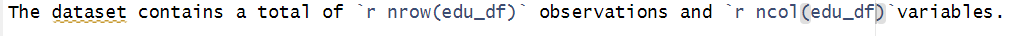
\includegraphics[keepaspectratio]{../images/inline_code.png}}

}

\caption{\label{fig-inlinecode}Inline R code}

\end{figure}%

See Figure~\ref{fig-inlinecode} for the detail of the \emph{Inline R
code} used.

\begin{table}

\caption{\label{tbl-tableone}First 2 rows of the data}

\centering{

\begin{Shaded}
\begin{Highlighting}[]
\FunctionTok{head}\NormalTok{(edu\_df\_selected, }\DecValTok{2}\NormalTok{)}
\end{Highlighting}
\end{Shaded}

\begin{verbatim}
# A tibble: 2 x 5
  income_flag              level3_at_18 uni_at_19 level6_at_22 size_flag  
  <chr>                           <dbl>     <dbl>        <dbl> <chr>      
1 Higher deprivation towns         50.8      30.8         NA   Small Towns
2 Mid deprivation towns            60.1      41.8         33.3 Small Towns
\end{verbatim}

}

\end{table}%

See Table~\ref{tbl-tableone} for the detail of the first 2 rows of the
data and the types of variables in the dataset.

\section{Methodology}\label{methodology}

\begin{Shaded}
\begin{Highlighting}[]
\NormalTok{edu\_df\_selected }\SpecialCharTok{\%\textgreater{}\%}
  \FunctionTok{count}\NormalTok{(income\_flag) }\SpecialCharTok{\%\textgreater{}\%}
  \FunctionTok{mutate}\NormalTok{(}\AttributeTok{percentage =} \FunctionTok{round}\NormalTok{(n }\SpecialCharTok{/} \FunctionTok{sum}\NormalTok{(n) }\SpecialCharTok{*} \DecValTok{100}\NormalTok{, }\DecValTok{1}\NormalTok{)) }\SpecialCharTok{\%\textgreater{}\%}
\NormalTok{  knitr}\SpecialCharTok{::}\FunctionTok{kable}\NormalTok{(}
    \AttributeTok{col.names =} \FunctionTok{c}\NormalTok{(}\StringTok{"Income Flag"}\NormalTok{, }\StringTok{"Count"}\NormalTok{, }\StringTok{"Percentage (\%)"}\NormalTok{),}
    \AttributeTok{digits =} \DecValTok{1}
\NormalTok{  )}
\end{Highlighting}
\end{Shaded}

\begin{longtable}[]{@{}lrr@{}}

\caption{\label{tbl-proportion_of_income}Proportion of Each Income Flag
Category}

\tabularnewline

\toprule\noalign{}
Income Flag & Count & Percentage (\%) \\
\midrule\noalign{}
\endhead
\bottomrule\noalign{}
\endlastfoot
Cities & 18 & 1.6 \\
Higher deprivation towns & 433 & 39.2 \\
Lower deprivation towns & 444 & 40.2 \\
Mid deprivation towns & 205 & 18.6 \\
NA & 4 & 0.4 \\

\end{longtable}

While reviewing the data (Table~\ref{tbl-proportion_of_income}), our
group discover that there is \textbf{missing data} (\texttt{NA} value)
in the income categories \texttt{income\_flag}. In order \textbf{not to
affect the accuracy of the subsequent analysis}, this missing data will
not be included in the analysis. Also, since the sample in
\texttt{Cities} of \texttt{income\_flag} is \textbf{too small and less
representative}, it is removed in the subsequent analysis.

\begin{Shaded}
\begin{Highlighting}[]
\NormalTok{edu\_df\_clean }\OtherTok{\textless{}{-}}\NormalTok{ edu\_df\_selected }\SpecialCharTok{\%\textgreater{}\%}
  \FunctionTok{filter}\NormalTok{(}\SpecialCharTok{!}\FunctionTok{is.na}\NormalTok{(income\_flag) }\SpecialCharTok{\&}\NormalTok{ income\_flag }\SpecialCharTok{!=} \StringTok{"Cities"}\NormalTok{) }\SpecialCharTok{\%\textgreater{}\%}
  \FunctionTok{mutate}\NormalTok{(}\AttributeTok{income\_flag =} \FunctionTok{factor}\NormalTok{(income\_flag,}
                              \AttributeTok{levels =} \FunctionTok{c}\NormalTok{(}\StringTok{"Higher deprivation towns"}\NormalTok{,}
                                         \StringTok{"Mid deprivation towns"}\NormalTok{,}
                                         \StringTok{"Lower deprivation towns"}\NormalTok{)))}
\end{Highlighting}
\end{Shaded}

\begin{Shaded}
\begin{Highlighting}[]
\NormalTok{table1 }\OtherTok{\textless{}{-}}\NormalTok{ edu\_df\_clean }\SpecialCharTok{\%\textgreater{}\%}
  \FunctionTok{group\_by}\NormalTok{(income\_flag) }\SpecialCharTok{\%\textgreater{}\%}
  \FunctionTok{summarise}\NormalTok{(}
    \AttributeTok{mean\_level3 =} \FunctionTok{mean}\NormalTok{(level3\_at\_18, }\AttributeTok{na.rm =} \ConstantTok{TRUE}\NormalTok{),}
    \AttributeTok{sd\_level3 =} \FunctionTok{sd}\NormalTok{(level3\_at\_18, }\AttributeTok{na.rm =} \ConstantTok{TRUE}\NormalTok{),}
    \AttributeTok{mean\_uni19 =} \FunctionTok{mean}\NormalTok{(uni\_at\_19, }\AttributeTok{na.rm =} \ConstantTok{TRUE}\NormalTok{),}
    \AttributeTok{sd\_uni19 =} \FunctionTok{sd}\NormalTok{(uni\_at\_19, }\AttributeTok{na.rm =} \ConstantTok{TRUE}\NormalTok{),}
    \AttributeTok{mean\_level6 =} \FunctionTok{mean}\NormalTok{(level6\_at\_22, }\AttributeTok{na.rm =} \ConstantTok{TRUE}\NormalTok{),}
    \AttributeTok{sd\_level6 =} \FunctionTok{sd}\NormalTok{(level6\_at\_22, }\AttributeTok{na.rm =} \ConstantTok{TRUE}\NormalTok{)}
\NormalTok{  ) }\SpecialCharTok{\%\textgreater{}\%}
  \FunctionTok{rename}\NormalTok{(}
    \StringTok{"Income Group"} \OtherTok{=}\NormalTok{ income\_flag,}
    \StringTok{"Mean: Level 3 at 18"} \OtherTok{=}\NormalTok{ mean\_level3,}
    \StringTok{"SD: Level 3 at 18"} \OtherTok{=}\NormalTok{ sd\_level3,}
    \StringTok{"Mean: HE at 19"} \OtherTok{=}\NormalTok{ mean\_uni19,}
    \StringTok{"SD: HE at 19"} \OtherTok{=}\NormalTok{ sd\_uni19,}
    \StringTok{"Mean: Level 6 at 22"} \OtherTok{=}\NormalTok{ mean\_level6,}
    \StringTok{"SD: Level 6 at 22"} \OtherTok{=}\NormalTok{ sd\_level6}
\NormalTok{  )}

\FunctionTok{kable}\NormalTok{(table1, }\AttributeTok{digits =} \DecValTok{2}\NormalTok{) }\SpecialCharTok{\%\textgreater{}\%}
  \FunctionTok{kable\_styling}\NormalTok{(}\AttributeTok{full\_width =} \ConstantTok{FALSE}\NormalTok{)}
\end{Highlighting}
\end{Shaded}

\begin{longtable}[t]{lrrrrrr}

\caption{\label{tbl-edu_means_by_income}Mean and SD of Educational
Outcomes by Income Group(Cities Excluded)}

\tabularnewline

\toprule
Income Group & Mean: Level 3 at 18 & SD: Level 3 at 18 & Mean: HE at 19 & SD: HE at 19 & Mean: Level 6 at 22 & SD: Level 6 at 22\\
\midrule
Higher deprivation towns & 41.59 & 7.35 & 27.13 & 6.69 & 23.99 & 4.92\\
Mid deprivation towns & 47.82 & 7.59 & 31.32 & 7.20 & 27.99 & 5.69\\
Lower deprivation towns & 57.96 & 9.68 & 40.78 & 10.33 & 35.68 & 8.33\\
\bottomrule

\end{longtable}

Table~\ref{tbl-edu_means_by_income} shows that \textbf{education
outcomes improve significantly at all measured stages as income levels
rise}.

For instance, the mean proportion of individuals achieving Level 3
qualifications by age 18 rises from \textbf{41.59\%} in \textbf{higher
deprivation} towns to \textbf{57.96\%} in \textbf{lower deprivation}
towns. Similar upward trends are observed for higher education
participation at age 19 (\textbf{27.13\%} to \textbf{40.78\%}) and for
achieving Level 6 qualifications by age 22 (\textbf{23.99\%} to
\textbf{35.68\%}).

\textbf{The standard deviations are relatively consistent across
groups}. This suggests that while variation exists, the overall
improvement in outcomes is not due to a small number of high performers.

\begin{Shaded}
\begin{Highlighting}[]
\NormalTok{edu\_long }\OtherTok{\textless{}{-}}\NormalTok{ edu\_df\_clean }\SpecialCharTok{\%\textgreater{}\%}
  \FunctionTok{pivot\_longer}\NormalTok{(}
    \AttributeTok{cols =} \FunctionTok{c}\NormalTok{(level3\_at\_18,}
\NormalTok{             uni\_at\_19,}
\NormalTok{             level6\_at\_22),}
    \AttributeTok{names\_to =} \StringTok{"education\_stage"}\NormalTok{,}
    \AttributeTok{values\_to =} \StringTok{"value"}
\NormalTok{  )}

\NormalTok{edu\_long}\SpecialCharTok{$}\NormalTok{income\_flag }\OtherTok{\textless{}{-}} \FunctionTok{recode}\NormalTok{(edu\_long}\SpecialCharTok{$}\NormalTok{income\_flag,}
  \StringTok{"Higher deprivation towns"} \OtherTok{=} \StringTok{"Higher}\SpecialCharTok{\textbackslash{}n}\StringTok{deprivation}\SpecialCharTok{\textbackslash{}n}\StringTok{towns"}\NormalTok{,}
  \StringTok{"Mid deprivation towns"} \OtherTok{=} \StringTok{"Mid}\SpecialCharTok{\textbackslash{}n}\StringTok{deprivation}\SpecialCharTok{\textbackslash{}n}\StringTok{towns"}\NormalTok{,}
  \StringTok{"Lower deprivation towns"} \OtherTok{=} \StringTok{"Lower}\SpecialCharTok{\textbackslash{}n}\StringTok{deprivation}\SpecialCharTok{\textbackslash{}n}\StringTok{towns"}
\NormalTok{)}

\NormalTok{edu\_long}\SpecialCharTok{$}\NormalTok{education\_stage }\OtherTok{\textless{}{-}} \FunctionTok{recode}\NormalTok{(edu\_long}\SpecialCharTok{$}\NormalTok{education\_stage,}
  \StringTok{"level3\_at\_18"} \OtherTok{=} \StringTok{"Level 3 at 18"}\NormalTok{,}
  \StringTok{"uni\_at\_19"} \OtherTok{=} \StringTok{"HE at 19"}\NormalTok{,}
  \StringTok{"level6\_at\_22"} \OtherTok{=} \StringTok{"Level 6 at 22"}
\NormalTok{)}

\FunctionTok{ggplot}\NormalTok{(edu\_long, }\FunctionTok{aes}\NormalTok{(}\AttributeTok{x =}\NormalTok{ income\_flag, }\AttributeTok{y =}\NormalTok{ value, }\AttributeTok{fill =}\NormalTok{ income\_flag)) }\SpecialCharTok{+}
  \FunctionTok{geom\_boxplot}\NormalTok{() }\SpecialCharTok{+}
  \FunctionTok{facet\_wrap}\NormalTok{(}\SpecialCharTok{\textasciitilde{}}\NormalTok{education\_stage, }\AttributeTok{scales =} \StringTok{"free\_y"}\NormalTok{) }\SpecialCharTok{+}
  \FunctionTok{labs}\NormalTok{(}\AttributeTok{x =} \StringTok{"Income Group"}\NormalTok{, }\AttributeTok{y =} \StringTok{"Proportion"}\NormalTok{) }\SpecialCharTok{+}
  \FunctionTok{theme\_minimal}\NormalTok{() }\SpecialCharTok{+}
  \FunctionTok{theme}\NormalTok{(}\AttributeTok{axis.text.x =} \FunctionTok{element\_text}\NormalTok{(}\AttributeTok{size =} \DecValTok{9}\NormalTok{, }\AttributeTok{lineheight =} \FloatTok{1.1}\NormalTok{))}
\end{Highlighting}
\end{Shaded}

\begin{figure}[H]

\centering{

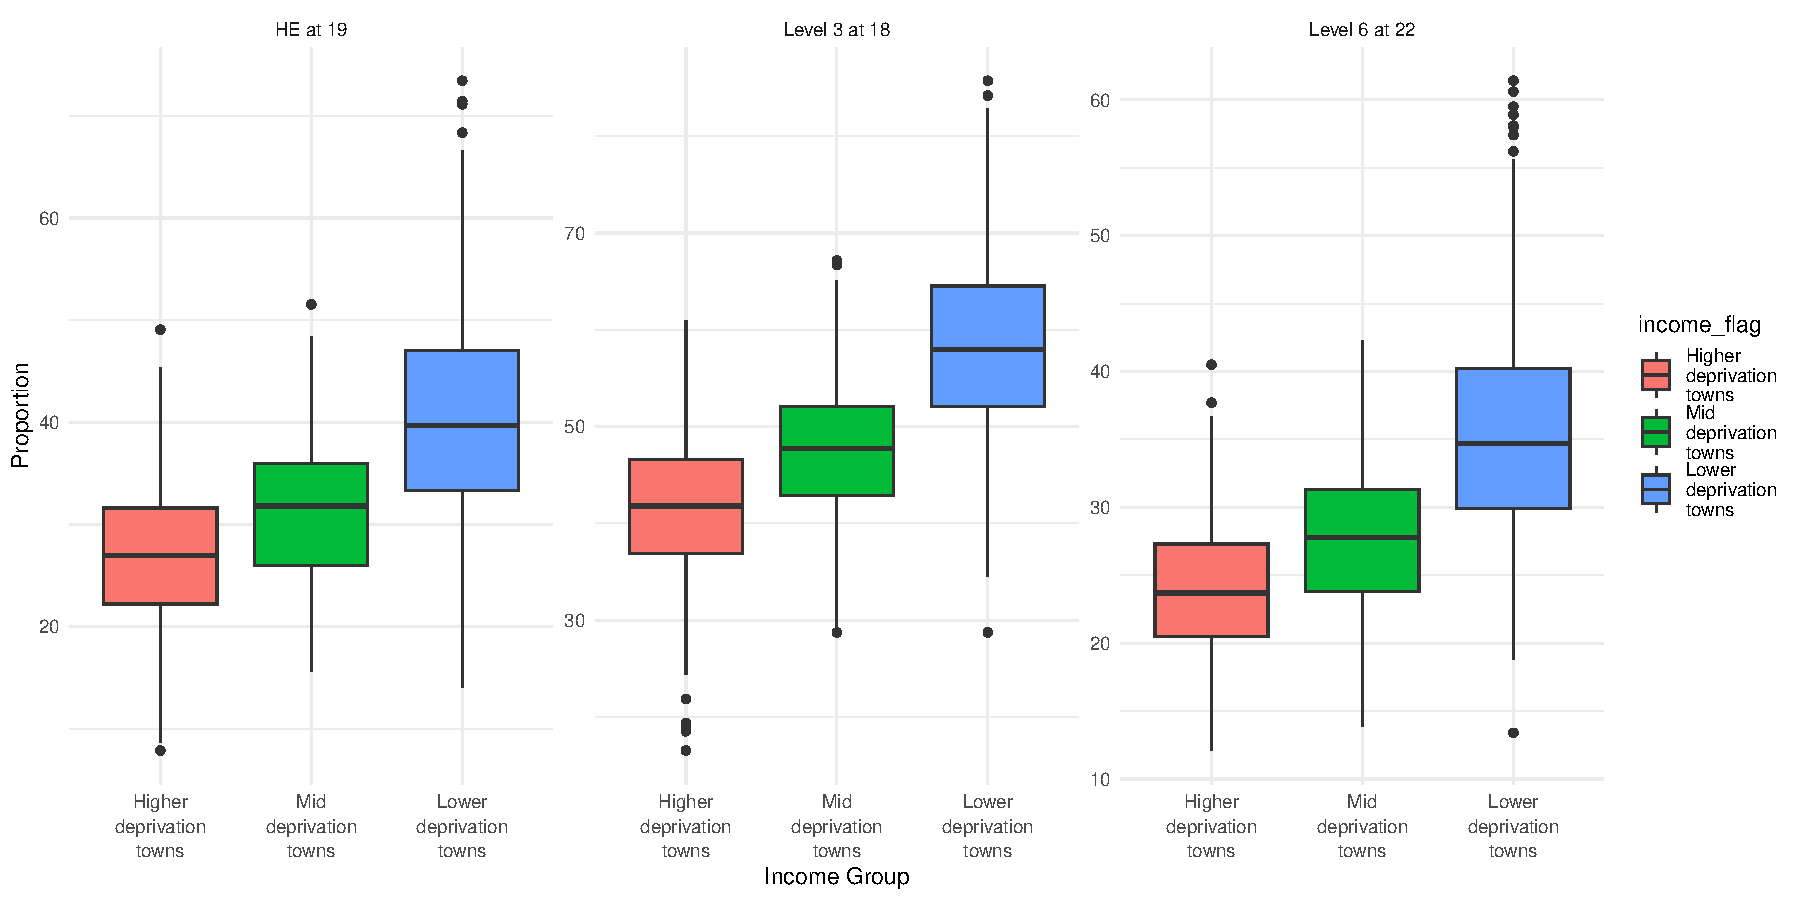
\includegraphics[width=1\linewidth,height=\textheight,keepaspectratio]{assignment3_files/figure-pdf/fig-edu_outcomes_boxplot-1.pdf}

}

\caption{\label{fig-edu_outcomes_boxplot}Educational Outcomes by Income
Group(Cities Excluded)}

\end{figure}%

Figure~\ref{fig-edu_outcomes_boxplot} illustrates \textbf{a clear upward
trend in educational attainment as town income levels increase}. In all
three stages, young people in lower deprivation towns consistently
outperform their peers in higher deprivation towns.

Specifically, the \textbf{median} proportions of youth achieving Level 3
qualifications at age 18, participating in full-time higher education at
age 19, and attaining Level 6 qualifications by age 22 are \textbf{all
higher in towns with lower deprivation}. The \textbf{interquartile
ranges} are also \textbf{narrower} in \textbf{lower deprivation} towns,
suggesting more consistent performance within these areas.

In contrast, \textbf{higher deprivation} towns exhibit not only
\textbf{lower median outcomes} but also \textbf{greater variability}, as
reflected by the wider spread of the boxplots and more outliers.

\section{Result}\label{result}

\begin{Shaded}
\begin{Highlighting}[]
\NormalTok{summary\_df }\OtherTok{\textless{}{-}}\NormalTok{ edu\_df\_clean }\SpecialCharTok{\%\textgreater{}\%}
  \FunctionTok{group\_by}\NormalTok{(income\_flag, size\_flag) }\SpecialCharTok{\%\textgreater{}\%}
  \FunctionTok{summarise}\NormalTok{(}
    \AttributeTok{level3 =} \FunctionTok{mean}\NormalTok{(level3\_at\_18, }\AttributeTok{na.rm =} \ConstantTok{TRUE}\NormalTok{),}
    \AttributeTok{uni19 =} \FunctionTok{mean}\NormalTok{(uni\_at\_19, }\AttributeTok{na.rm =} \ConstantTok{TRUE}\NormalTok{),}
    \AttributeTok{level6 =} \FunctionTok{mean}\NormalTok{(level6\_at\_22, }\AttributeTok{na.rm =} \ConstantTok{TRUE}\NormalTok{)}
\NormalTok{  ) }\SpecialCharTok{\%\textgreater{}\%}
  \FunctionTok{pivot\_longer}\NormalTok{(}
    \AttributeTok{cols =} \FunctionTok{c}\NormalTok{(level3, uni19, level6),}
    \AttributeTok{names\_to =} \StringTok{"education\_stage"}\NormalTok{,}
    \AttributeTok{values\_to =} \StringTok{"mean\_value"}
\NormalTok{  )}

\NormalTok{summary\_df}\SpecialCharTok{$}\NormalTok{education\_stage }\OtherTok{\textless{}{-}} \FunctionTok{recode}\NormalTok{(summary\_df}\SpecialCharTok{$}\NormalTok{education\_stage,}
  \StringTok{"level3"} \OtherTok{=} \StringTok{"Level 3 at Age 18"}\NormalTok{,}
  \StringTok{"uni19"} \OtherTok{=} \StringTok{"University at 19"}\NormalTok{,}
  \StringTok{"level6"} \OtherTok{=} \StringTok{"Level 6+ by Age 22"}
\NormalTok{)}

\NormalTok{summary\_df}\SpecialCharTok{$}\NormalTok{income\_flag }\OtherTok{\textless{}{-}} \FunctionTok{recode}\NormalTok{(summary\_df}\SpecialCharTok{$}\NormalTok{income\_flag,}
  \StringTok{"Higher deprivation towns"} \OtherTok{=} \StringTok{"Higher}\SpecialCharTok{\textbackslash{}n}\StringTok{deprivation}\SpecialCharTok{\textbackslash{}n}\StringTok{towns"}\NormalTok{,}
  \StringTok{"Mid deprivation towns"} \OtherTok{=} \StringTok{"Mid}\SpecialCharTok{\textbackslash{}n}\StringTok{deprivation}\SpecialCharTok{\textbackslash{}n}\StringTok{towns"}\NormalTok{,}
  \StringTok{"Lower deprivation towns"} \OtherTok{=} \StringTok{"Lower}\SpecialCharTok{\textbackslash{}n}\StringTok{deprivation}\SpecialCharTok{\textbackslash{}n}\StringTok{towns"}
\NormalTok{)}

\FunctionTok{ggplot}\NormalTok{(summary\_df, }\FunctionTok{aes}\NormalTok{(}\AttributeTok{x =}\NormalTok{ income\_flag, }\AttributeTok{y =}\NormalTok{ mean\_value, }\AttributeTok{fill =}\NormalTok{ education\_stage)) }\SpecialCharTok{+}
  \FunctionTok{geom\_col}\NormalTok{(}\AttributeTok{position =} \StringTok{"dodge"}\NormalTok{, }\AttributeTok{width =} \FloatTok{0.7}\NormalTok{) }\SpecialCharTok{+}
  \FunctionTok{facet\_wrap}\NormalTok{(}\SpecialCharTok{\textasciitilde{}}\NormalTok{size\_flag) }\SpecialCharTok{+}
  \FunctionTok{labs}\NormalTok{(}
    \AttributeTok{x =} \StringTok{"Income Deprivation Group"}\NormalTok{,}
    \AttributeTok{y =} \StringTok{"Average Proportion"}\NormalTok{,}
    \AttributeTok{fill =} \StringTok{"Education Stage"}
\NormalTok{  ) }\SpecialCharTok{+}
  \FunctionTok{scale\_fill\_manual}\NormalTok{(}
    \AttributeTok{values =} \FunctionTok{c}\NormalTok{(}
      \StringTok{"Level 3 at Age 18"} \OtherTok{=} \StringTok{"\#4C72B0"}\NormalTok{,}
      \StringTok{"University at 19"} \OtherTok{=} \StringTok{"\#55A868"}\NormalTok{,}
      \StringTok{"Level 6+ by Age 22"} \OtherTok{=} \StringTok{"\#C44E52"}
\NormalTok{    )}
\NormalTok{  ) }\SpecialCharTok{+}
  \FunctionTok{theme\_minimal}\NormalTok{() }\SpecialCharTok{+}
  \FunctionTok{theme}\NormalTok{(}\AttributeTok{axis.text.x =} \FunctionTok{element\_text}\NormalTok{(}\AttributeTok{size =} \DecValTok{9}\NormalTok{, }\AttributeTok{lineheight =} \FloatTok{1.1}\NormalTok{))}
\end{Highlighting}
\end{Shaded}

\begin{figure}[H]

\centering{

\centering{

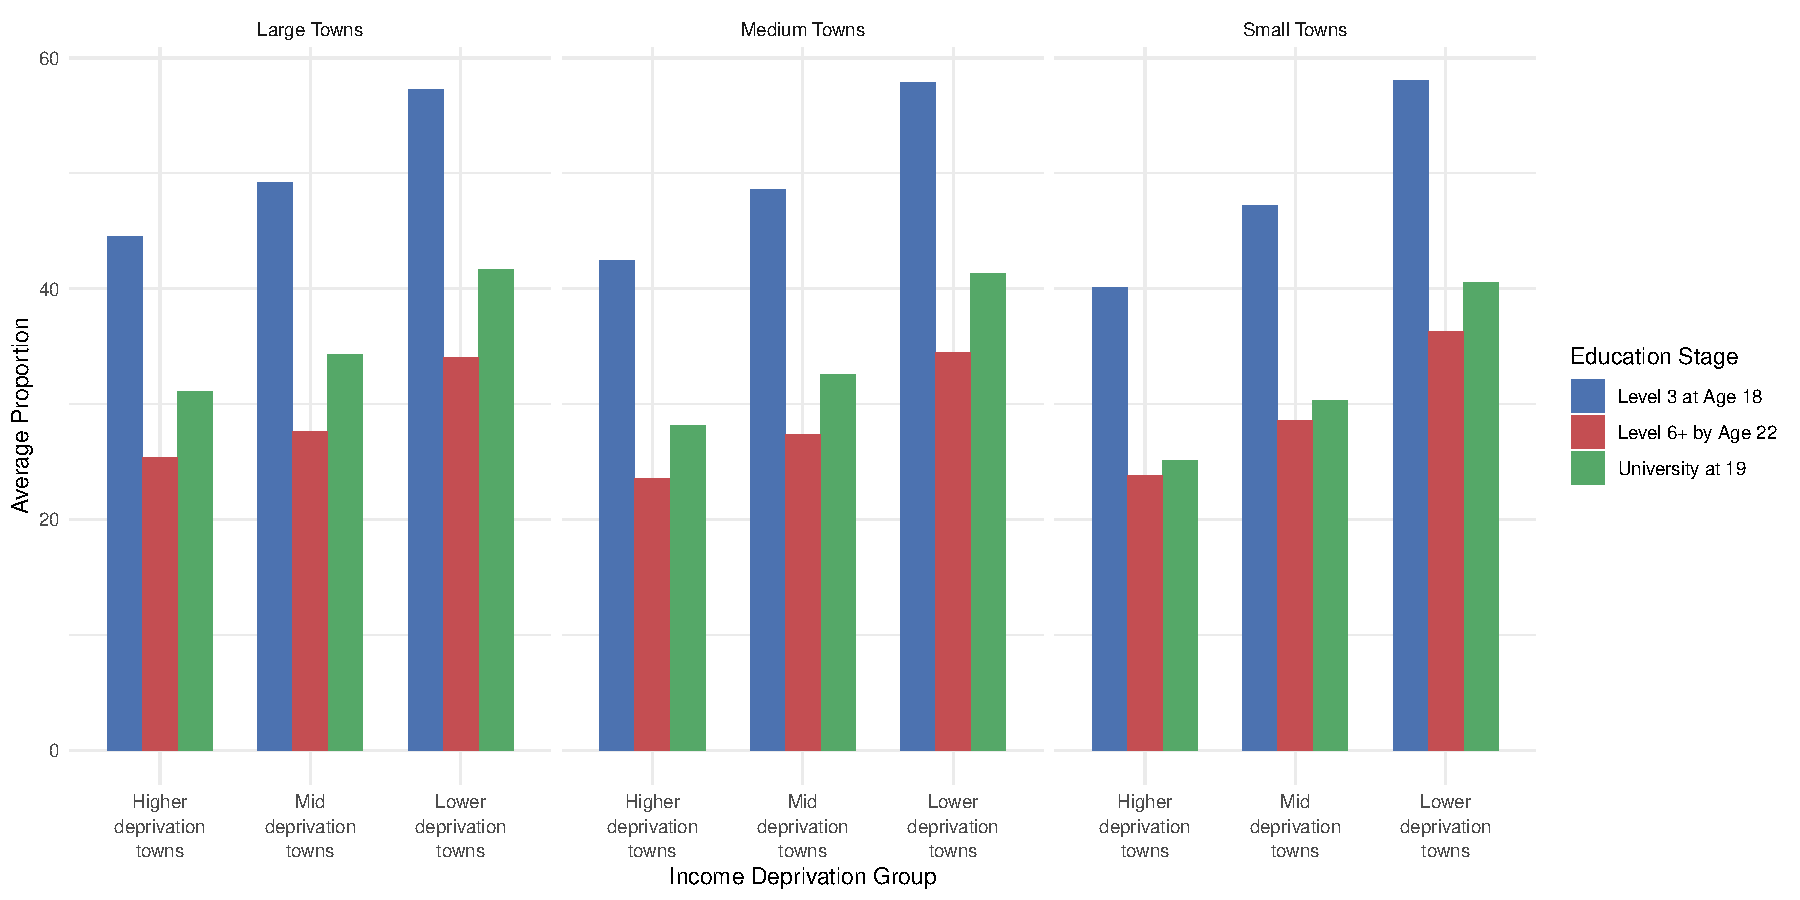
\includegraphics[width=1\linewidth,height=\textheight,keepaspectratio]{assignment3_files/figure-pdf/fig-income-education-by-size-1.pdf}

}

\subcaption{\label{fig-income-education-by-size}Comparison of
educational outcomes across income levels and town sizes}

}

\caption{\label{fig-income-education-by-size}Educational Attainment by
Income Deprivation Level and Town Size (Cities Excluded)}

\end{figure}%

As shown in Figure~\ref{fig-income-education-by-size},
\textbf{educational attainment increases consistently as income
deprivation decreases, across all town sizes}. Towns with \textbf{lower
deprivation levels} demonstrate the \textbf{highest average proportions}
of students achieving Level 3 qualifications at age 18, entering
university at age 19, and obtaining Level 6 or higher qualifications by
age 22.

This pattern holds for large, medium, and small towns, though the gap
between high and low deprivation groups appears most pronounced in small
towns, particularly at the Level 6+ stage. In small towns, the
difference in university attainment between high and low deprivation
groups exceeds 10 percentage points.

These results \textbf{reinforce a strong association between local
income levels and youth educational outcomes}, and suggest that
deprivation may have an even stronger impact in smaller towns.

\section{Discussion}\label{discussion}

Our analysis reveals a consistent trend: towns with lower levels of
income deprivation demonstrate stronger educational outcomes at ages 18,
19, and 22. This association holds across all town sizes and is
particularly pronounced in smaller towns, where the disparity in Level 6
qualifications is most significant. These findings align with recent
research by the UK Office for National Statistics (ONS), which suggests
that less deprived areas may offer more supportive conditions for
academic progression.

Nonetheless, several limitations of this study must be acknowledged.
First, as an observational analysis, our findings illustrate correlation
rather than causation. While the relationship between deprivation and
lower attainment is strong, we cannot definitively claim that income
deprivation directly causes poorer educational outcomes. Second, the use
of broad categorical income groupings may mask finer-grained local
differences, potentially obscuring key contextual factors. Third, we
deliberately excluded cities to ensure analytical consistency; however,
this decision limits the generalisability of our findings, particularly
to urban populations who often face distinct educational barriers.
Lastly, the dataset is limited to a single cohort of students from the
2012/13 academic year, meaning it may not capture evolving socioeconomic
dynamics or long-term trends in educational performance.

Despite these constraints, the findings clearly highlight structural
inequalities that disadvantage youth in more deprived towns. This
underscores the need for targeted, evidence-based policy interventions
to reduce educational disparities. Future research should incorporate
longitudinal data and more granular socioeconomic indicators to deepen
our understanding of these patterns and inform more effective policy
responses.

\section{Conclusion}\label{conclusion}

This study found a clear relationship between \textbf{income
deprivation} and \textbf{young people's educational attainment} at town
level in England. At all three stages of education, young people from
\textbf{less deprived towns} and cities consistently
\textbf{outperformed} those from more deprived areas. This trend exists
across towns and cities of all sizes, and is particularly evident in
\textbf{smaller towns}. While the findings are consistent with national
statistics and highlight structural inequalities, \textbf{caution should
be exercised in interpreting the results} due to the observational
nature and limited scope of the study.

\section{Recommendations}\label{recommendations}

To address the disparities observed, education policy should
\textbf{prioritize support for students in high-deprivation towns}. This
may include:

\begin{itemize}
\item
  Enhance educational funding and targeted support in high-deprivation
  towns
\item
  Expand access programs to encourage university progression
\item
  Better access to higher education pathways
\item
  Integrate deprivation indicators into education planning and policy to
  ensure equitable resource distribution
\end{itemize}

In addition, \textbf{future research} should expand the study's dataset.
There is a need to include \textbf{multiple clusters and urban areas}
and to \textbf{integrate qualitative indicators} such as school quality
and student support services as study variables. These efforts will
contribute to \textbf{a more comprehensive understanding of how income
poverty affects educational trajectories} and inform the development of
more equitable education strategies.

\section{Citation}\label{citation}

\textbf{R and R Package}

\begin{enumerate}
\def\labelenumi{\arabic{enumi}.}
\item
  R Core Team (2025). \emph{R: A Language and Environment for
  Statistical Computing}. R Foundation for Statistical Computing,
  Vienna, Austria. \url{https://www.R-project.org/}.
\item
  Wickham H, François R, Henry L, Müller K, Vaughan D (2023).
  \emph{dplyr: A Grammar of Data Manipulation}. R package version 1.1.4,
  \url{https://CRAN.R-project.org/package=dplyr}.
\item
  H. Wickham. ggplot2: Elegant Graphics for Data Analysis.
  Springer-Verlag New York, 2016.
\item
  Wickham H, Hester J, Bryan J (2024). \emph{readr: Read Rectangular
  Text Data}. R package version 2.1.5,
  \url{https://CRAN.R-project.org/package=readr}.
\item
  Wickham H, Vaughan D, Girlich M (2024). \emph{tidyr: Tidy Messy Data}.
  R package version 1.3.1,
  \url{https://CRAN.R-project.org/package=tidyr}.
\item
  Xie Y (2024). \emph{knitr: A General-Purpose Package for Dynamic
  Report Generation in R}. R package version 1.49,
  \url{https://yihui.org/knitr/}.

  Yihui Xie (2015) Dynamic Documents with R and knitr. 2nd edition.
  Chapman and Hall/CRC. ISBN 978-1498716963

  Yihui Xie (2014) knitr: A Comprehensive Tool for Reproducible Research
  in R. In Victoria Stodden, Friedrich Leisch and Roger D. Peng,
  editors, Implementing Reproducible Computational Research. Chapman and
  Hall/CRC. ISBN 978-1466561595
\item
  Zhu H (2024). \emph{kableExtra: Construct Complex Table with `kable'
  and Pipe Syntax}. R package version 1.4.0,
  https://github.com/haozhu233/kableExtra,
  \url{http://haozhu233.github.io/kableExtra/}.
\end{enumerate}

\textbf{Data Used}

\begin{enumerate}
\def\labelenumi{\arabic{enumi}.}
\item
  Office for National Statistics. (2023, July 25). \emph{Why do children
  and young people in smaller towns do better academically than those in
  larger towns?}

  \url{https://www.ons.gov.uk/peoplepopulationandcommunity/educationandchildcare/articles/whydochildrenandyoungpeopleinsmallertownsdobetteracademicallythanthoseinlargertowns/2023-07-25}
\item
  The Times. (2024, August 14). University offers at record high as
  inequality in degree entry grows. Retrieved from
  \url{https://www.thetimes.co.uk/article/university-offers-at-record-high-as-inequality-in-access-grows-ttj9scz6b}
\end{enumerate}

\end{document}
